首先分治的做法是众所周知的.

有期望$O(n)$的随机增量法: 首先将所有点随机打乱, 然后每次增加一个点, 更新答案.

假设当前最近点对距离为$s$, 则把平面划分成$s \times s$的方格, 用哈希表存储每个方格有哪些点.

加入一个新点时只需要枚举自身和周围共计$9$个方格中的点, 显然枚举到的点最多$16$个. 如果加入之后答案变小了就$O(n)$暴力重构.

前$i$个点中$i$是最近点对中的点的概率至多为$\frac 2 i$, 所以每个点的期望贡献都是$O(1)$, 总的复杂度就是期望$O(n)$.

如果对每个点都要求出距离最近的点的话, 也有随机化的$O(n)$做法:

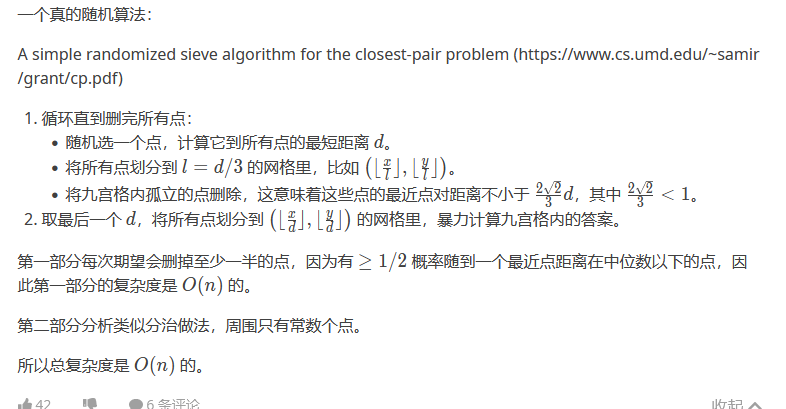
\includegraphics[scale=0.5]{../src/geometry/最近点对.png}